\chapter{LAMPIRAN}
\label{chap:lampiran}

\section*{Hasil Simulasi Saat Ini}
\label{sec:hasil-simul-existing}

\begin{figure}[!ht]
    \centering
    % First row - two images side by side
    \begin{subfigure}{0.48\textwidth}
        \centering
        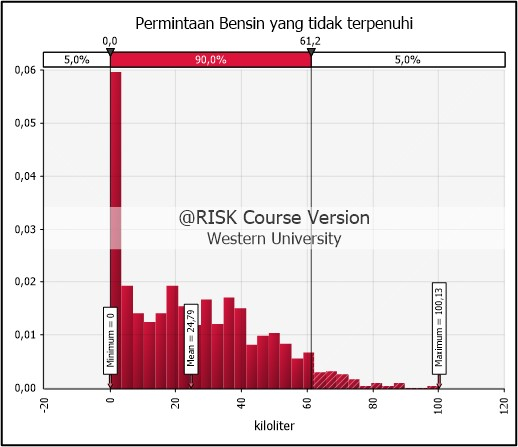
\includegraphics[width=\textwidth]{grafik/minus-bensin-saat-ini.jpg}
        \caption{Bensin}
        \label{fig:minus-bensin-saat-ini}
    \end{subfigure}
    \hfill
    \begin{subfigure}{0.48\textwidth}
        \centering
        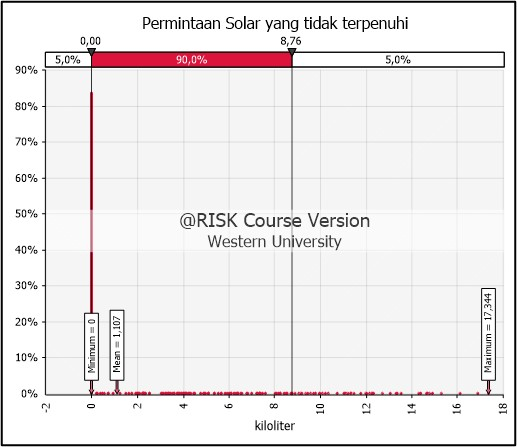
\includegraphics[width=\textwidth]{grafik/minus-solar-saat-ini.jpg}
        \caption{Solar}
        \label{fig:minus-solar-saat-ini}
    \end{subfigure}
    
    \vspace{1cm}  % Add vertical space between rows
    
    % Second row - single image centered
    \begin{subfigure}{0.5\textwidth}
        \centering
        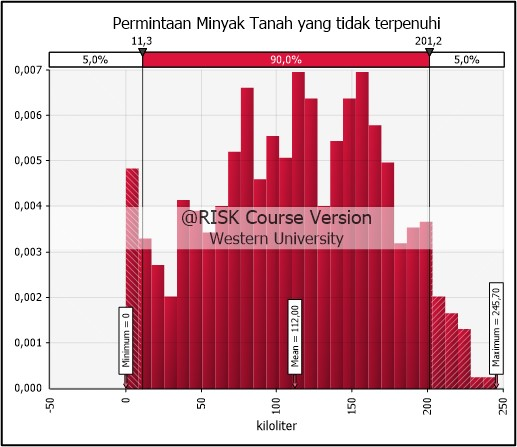
\includegraphics[width=\textwidth]{grafik/minus-mt-saat-ini.jpg}
        \caption{Minyak Tanah}
        \label{fig:minus-mt-saat-ini}
    \end{subfigure}
    \caption{Permintaan BBM yang Tidak Terpenuhi Saat Ini}
    \label{fig:minus-bbm-saat-ini}
\end{figure}

\begin{figure}[!ht]
    \centering
    \begin{subfigure}{0.48\textwidth}
        \centering
        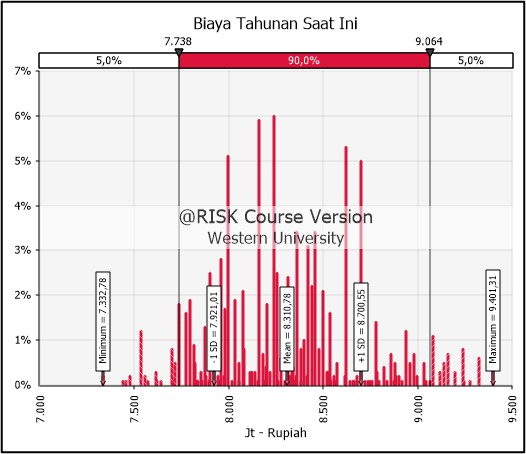
\includegraphics[width=\textwidth]{grafik/biaya-tahunan-saat-ini.jpg}
    \end{subfigure}
    \hfill  % This adds horizontal spacing between images
    \begin{subfigure}{0.48\textwidth}
        \centering
        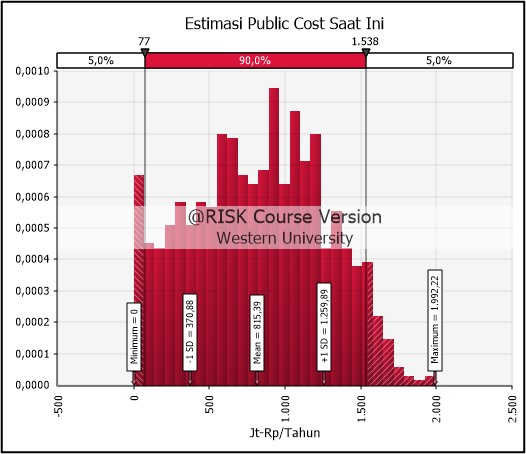
\includegraphics[width=\textwidth]{grafik/biaya-publik-saat-ini.jpg}
    \end{subfigure}
    \caption{Hasil Simulasi Biaya Saat Ini}
    \label{fig:biaya-saat-ini}
\end{figure}

% \section*{Hasil Simulasi Saat Ini}
% \label{sec:hasil-simul-existing}


